\documentclass[a4paper,10pt]{article}

%\usepackage[utf8]{inputenc}
\usepackage[top=2cm, bottom=2cm, left=2cm, right=2cm]{geometry}

\usepackage{graphicx} %%For loading graphic files
\usepackage{hyperref}
\graphicspath{ {Pics/} }
%\DeclareGraphicsExtensions{.png,.pdf}


\begin{document}


\title{Global Audio Manager Manual}
\author{Baranger - Holsnyder}
%\date{} %%If commented, the current date is used.
\maketitle

\clearpage


\tableofcontents %Table of contents

\clearpage



\section*{Introduction}

GAM is a set of tools designed to optimize and speed up audio integration.

\section{Arborescence}

A file hierarchy has been set up within a \emph{Resources} subfolder to allow for an optimized, faster audio integration in your Unity project. This hierarchy represents a conform audio structure, split into three domains : Voice, Sound Effects (SFX) and Music (see \autoref
{sec:gen}).


\section{Audio Clip Manager}

Access : Menu Windows/Global Audio Manager/GAMAudioClipManager
\\

The Audio Clip Manager is a file browser designed specifically to allow a global view of all audio assets and optimize their management. All audio import settings associated with an AudioClip (actually the same ones as in the regular AudioClip inspector view), along with platform-specific options, can be managed from here. This becomes indispensable when working on projects ranging from medium-size to maddening large. \\

AudioClips are split into 3 audio types (Music, SFX and Voices. See \nameref{sec:gen} section for more info). This separation is extremely useful for giving type-specific values to audio import settings of whole batches of clips. All import settings should be type-specific to allow maximum quality to performance proportion at runtime. \
Clips corresponding to each type can be viewed separately, or all can be show together ; a fifth option allows to show all typeless clips. This can be managed with the 5 buttons on the left-hand side of the toolbar. This separation can be defined manually, by assigning singular or batches of AudioClips to a type (to select an array of clips, use the shift key or control(PC)/command(Mac) key), or automatically, provided the name of the type appears somewhere along the project-relative file path.\\

On the right side of the toolbar, an array (or drop-down menu) of gaming platforms is represented. By selecting a platform, you can edit the import settings for it, independently from the others. Or make it follow the default pattern. \\

The browser view itself imitates the regular Unity browser view, each line representing an AudioClip, and columns - its settings for various runtime and import parameters. Modifying a setting for an AudioClip within a selection will modify the setting in the same manner for all selected clips. 
%The paramaters are as follows : 
%\begin{itemize}
%\item To Mono : force a clip into a mono configuration. This transforms a multichannel audio clip into a mono clip at runtime. Such a reduction can bypass issues with left/right panning inside an AudioClip, like a wrong panning.
%
%\item Background Load
%
%\item Preload :
%
%\item Load Type : 
%
%\item Format : the audio codec used for the audioclip. Allows changes on the quality/file size scale. Recommended : Vorbis, with type-specific quality settings (see below).
%
%\item Quality : compression rate of a compressed audioclip. The higher the quality, the lower the compression. Recommended optimal compression with minimal quality loss : \textasciitilde 80\% for music, \textasciitilde 40\% for SFX and \textasciitilde 70\% for voices. These numbers can greatly vary depending on the considered sounds, their pre-compression quality and the desired post-compression quality.
%
%\item Sample Rate : In a similar manner to quality, allows file size reduction at the price of data loss. Use very carefully ! As a general rule, do not assign a sample rate value lower than 44.100 Hz, and rely on the the \textit{Preserve} and \textit{Optimize} options.
%
%\item Label : the type (Music/SFX/Voice) of the clip.
%\end{itemize}
%
%Right-clicking a selection of AudioClips allows tweaking more parameters :...


\section{UI}

The UI Utility automatically references all the UI objects which are liable to play a sound on user interaction\footnote{Components derived from the Selectable class.}, and allows to define and control these sounds and their playback settings.

\subsection{GAM UI Editor}
\textbf{Access} : Menu Windows/Global Audio Manager/GAMUI\\

This window allows a global overview of all selectable objects within the project, or under a specific canvas. It is split horizontally into three sections.

\subsubsection{Events-sounds assignments}
The top section allows building a \emph{setting}, which is basically a list of UI Events paired to Switches (see \nameref{sec:switch} section). All possible UI events are available.\\

This setting can in turn be applied (Apply setting button) to all UI objects referenced in the \nameref{subsec:objove}. \
On the contrary, the Clear objects of events button will delete all relevant\footnote{Meaning events which trigger a switch} events on these objects.

\subsubsection{Parent objects}
The \emph{parent objects} determine where to look for UI game objects. Canvases containing UI objects can be referenced using the + button, or all can be automatically added using the Add canvases in scene button.

\subsubsection{Objects Overview}\label{subsec:objove}
All referenced UI objects and all their relevant\footnote{Meaning events which trigger a switch} UI events are shown here.


\section{Music}

\subsection{GAMMusic window}
\textbf{Access} : Menu Windows/Global Audio Manager/GAMMusic\\

Allows integration of dynamic music, from simple setups to complex interactive systems. Small musical cells are fed into GAMMusic (possibly with separate instruments), and a complete dynamic music can be built.

\subsubsection{Parts}
These elements are the reservoir side of music building, or the vertical assembling. They can be managed from the lower part of the window. All elements within this section can be activated and deactivated (and will respectively be taken in consideration during playback or ignored).\

\paragraph{Cells: } Music \emph{cells} are the smallest building block of a music. They represent a short length of music, and either a slice of the whole music, or a slice of an instrumental track. Cells should be made in different versions\footnote{One can use humanized quantization options on MIDI files to achieve realism. An audio recording should be made several times to produce different versions.}, and during playback one of these will be picked randomly (in the manner of a simplified \nameref{sec:switch}) by the \emph{track} container.

\paragraph{Track: } these contain similar cells (the several versions mentioned above). They are in turn summed by the \emph{part}. They can be faded in and out.

\paragraph{Part: } A part contains several instruments, and will play them together (and each one will pick a cell version, if any). It represents the total vertical slice of music. These are the basic building blocks for \emph{structuring }music.\\

The menu in the purple toolbar allows loading AudioClips with respect to folder structure : Selecting a folder containing directories and subdirectories following the above hierarchy will load them into the music. The folder structure should be : Music folder/Part/Track/Cell.wav.

\subsubsection{Structures}
Structures are the instantiation of elements of the reservoir side, also named horizontal assembling. They are managed from the top part of the window.\\
The menu in the purple toolbar allows switching structures or adding new ones.

\paragraph{Structure: } a chain of parts. Each part in a chain can be looped (special instructions must then be sent to beak out of the loop). Each structure will be looped unless a follow-up is triggered.

\subsubsection{Mixes}
Mixes interact with both \emph{parts} and \emph{structures} and are the actual way of playing a music : a mix references a structure, and a setup of parts elements activations and fades. They can be managed from the left-hand side panel in the window.\\

The menu in the purple toolbar allows adding mixes.

\subsubsection{GAMMusic file}
All of the above should be \textbf{saved} into a special asset - a music file. The top-most purple toolbar allows all usual interactions on a file : opening, saving, saving as, creating a new one...


\subsection{GAMMusic Component}
This is the component which is used to actually play a music at runtime. It simply references a music file, and various functions in it allow interacting with it from other scripts.


%Easy integration of a mono or stereo dynamic music. \
%The example shows the structural slicing of an 8-bit version of the Tetris music. \
%More advanced options can be used to create a multitrack randomized music with the same slicing method. The example shows the process of creating such a music from a gypsy-jazz version of the same Tetris music.


\section{Switch} \label{sec:switch}

\subsection{Quick theory}
The fundamental tool of the sound designer. The switch allows for variation on sound samples, and is frequently used on any sound that occurs more than once. Without this, the game inevitably sounds artificial and poor.\\

The switch is at its core an array of similar AudioClips (for example, several footstep sounds for the same character walking on a given material) ; when playing a sound, instead of directly calling an AudioClip, a switch containing the AudioClip and its variations should be called. The switch will then randomly choose one of its AudioClips and play it.

\subsection{Switch creation and setup}

In GAM, the switch is an asset, created in a similar manner to any other asset : right-click in the browser view. Doing this with folders or AudioClips selected will create a switch referencing the selected AudioClips and the ones under the selected directories. \\

The user has a great amount of control over the playback of a switch, which allows for a limitless sound variation potential.
	\begin{itemize}
	\item \textbf{Presets} include Music, Sound Effects and UI and setup the parameters of your switch to adequate values. This should be used carefully though, and requires checking, as all sounds won't react in the same manner to the possible changes.
	\item \textbf{Play On Start} matches the option on the AudioSource.
	\item \textbf{2D/3D} actually matches the spatial blend in an AudioSource, and will override it with the boundary values on the scale.
	\item \textbf{2D/3D}
	\item \textbf{Volume} is self-explanatory. It will scale the volume for all the contained AudioClips.
	\item \textbf{Loop Policy} handles the way the AudioClips will be played when the switch is triggered. 
		\begin{itemize}
		\item \emph{One shot} Picks a clip and plays it.
		\item \emph{Repeat} will continuously play the contained AudioClips, picking one when one finished. This setting and the following one are useful for audio backgrounds.
		\item \emph{Repeat and exclude last element} will also continuously play the contained AudioClips, but will not play the same one twice in a row.
		\end{itemize}
	\item \textbf{Fade} handles fade-ins and fade-outs. If ticked, fade-in and fade-out durations below will be applied to switch playback (at the beginning and at the end of the switch, respectively, whether playback is looped or one-shot).
	\item \textbf{Random pitch} randomizes the pitch of an AudioClip when it is played. The values displayed are in semitones. The randomization range is represented by the min-max slider. This can be especially useful for footsteps and other repetitive small impacts.
	%\item \textbf{Delay} ????????????????????
	\item \textbf{Element} is the name given to the referenced AudioClips, as they have slightly increased functionality : they are weighted. That's the slider on the left of each AudioClip line. Weight works like a normal, statistical/randomization weight : the higher it is, the more chances the AudioClip has of being picked at playback. A weight of 0 will prevent the AudioClip from being picked.
	\item \textbf{Add Audio from directory} allows to add all AudioClips in a directory.
	\end{itemize}

\subsection{Integration: Switch component}
Since the switch extends the regular AudioClip/AudioSource functionality, it has its own component for integration : the \textbf{GAMSwitchComponent}, under Scripts. It allows referencing an existing switch and edit its settings (with the same interface as the own for the asset inspector). A Switch Component should have its own GameObject to avoid any AudioSource conflict with another Audio component. \\
The switch can handle AudioSource creation, but creating one for each switch component is recommended for more flexibility (the AudioSource still has some options the switch is missing, especially the tracks routing).


\section{Animation}

\textbf{Access} : Menu Windows/Global Audio Manager/GAMAnimation\
Or via GAMAnimation component.\\

Utilities allowing in-editor animation preview with sound and sound event addition and synchronization on the animation timeline. This utility allows for a classic \textit{play switch} event (see \autoref{sec:switch}), or for a \textit{play switch on surface} event, which automatically detects the surface under the animated object and plays a corresponding switch. The latter can typically be used for automatic surface-dependent footstep sounds on animated characters. \\
Two buttons on the left-hand side of the toolbar allow to switch views between Animation and Footsteps.

\subsection{GAM Animation Component}

\subsection{Animation view}
A global view of all Animation Clips present in the project. Mainly useful for 3D animations : Unity's 2D animation preview isn't handled well and can be completed with any sprite animation preview package on the asset store (beware though, some of these plugins may break the 3D animations preview). 3D animations require an avatar to generate a preview.\\



\subsection{Footsteps view}



\section{Generalities} \label{sec:gen}

Audio design in a video game is made up of several layers : \begin{itemize}
\item Music.
\item Environment Sound Effects : 
	\begin{itemize}
	\item Background : non-spatialized, 2D sounds.
	\item Objects : spatialized, 3D sounds.
	\end{itemize}
\item Action SFX.
\item UI SFX.
\item Voices.
\end{itemize}


\subsection{Non-spatialized sounds}
Unity calls these 2D sounds. DO NOT mistake that for a 2D-game-exclusive instruction. Both 2D and 3D sounds should be used for any Unity project. \
A non-spatialized sound is played back directly by the sound engine, without any processing from Unity, exactly like if it were played by a regular media player. This setting is often (but not systematically) used for music, voices and background SFX. \\

\paragraph{Example} : A garden with \emph{birds} in the \emph{trees} and a \emph{fountain} in the center.\
Background audio : Birds in the trees. More or less present depending on the time of day.

\subsection{Fixed spatialized sounds}
Fixed spatialized sounds are used for objects which don't move. Nevertheless, if the listener moves, their volume will change accordingly.

\paragraph{Example} : A garden with \emph{birds} in the \emph{trees} and a \emph{fountain} in the center.\
Fixed spatialized sound : the fountain. It emits sound, and the player can get closer or farther. So the fountain will have an audio source, with a volume rolloff curve. For a classic, realistic rolloff, the curve should be an invert-type function.\

%\begin{figure}[h]
%\centering
%\caption{2D object rolloff.}
%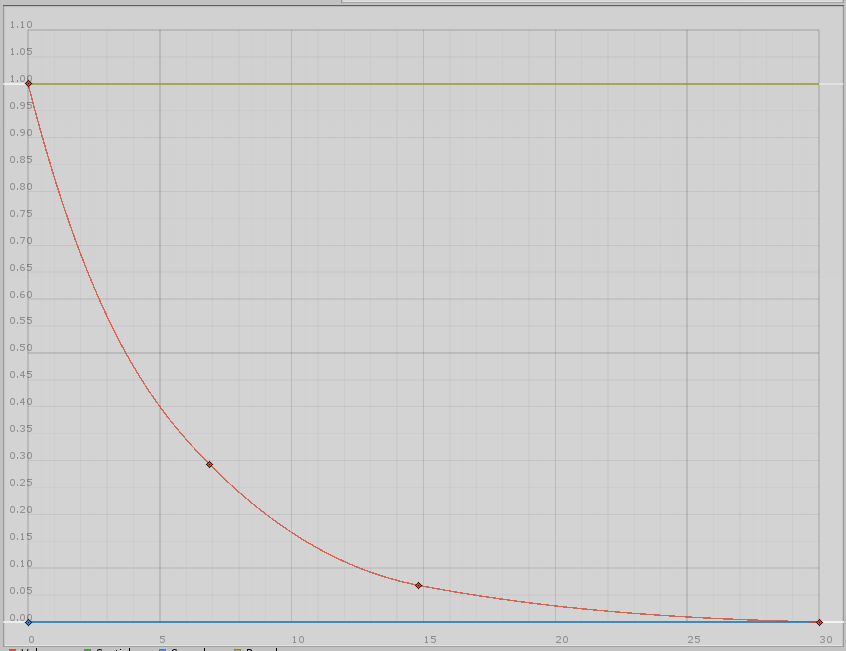
\includegraphics[width=0.5\linewidth]{logRolloff}
%\end{figure}



\subsection{Mobile spatialized sounds}
A spatialized sound may be attached to a moving object.
\paragraph{Example: } A garden with \emph{birds} in the \emph{trees} and a \emph{fountain} in the center.\
A crow passes overhead and sticks around. To achieve realism, 3 elements are necessary :

\begin{itemize}
\item A switch with 2 cawing sounds at the least.
\item A Doppler effect to add to the feeling of changing distance.
\item A volume rolloff of the type :\
\end{itemize}

%\begin{figure}[h]
%\centering
%\caption{Invert function rolloff.}
%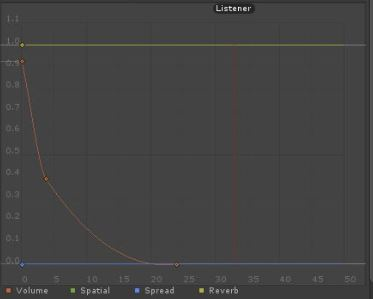
\includegraphics[width=0.4\linewidth]{dopplerRolloff}
%\end{figure}

%\appendix
%This is a useless appendix

\end{document}

